Camera calibration is the process of finding out the intrinsic, extrinsic parameters and the distortion coefficients. One of their uses is removing distortion. \\
Calibration is based on solving basic geometrical equations based on a chosen calibrating object. We detect the corners of the pattern. Most common are ChArUco patterns. ChArUco patterns are made up of chessboard and ArUco patterns. ArUco markers have fast detection but their accuracy is not high. Chessboards have a greater accuracy because each corner is surrounded by two black squares but the it has to be completely visible and its harder to detect. By combining these two we get the best of both of them. With the ArUco markers we can interpolate the positions of chessboard corners which allows partial views. Also because of the ArUco markers, each chessboard corner can have a unique id not dependent on if the pattern is rotated. 

\begin{figure}[h]
    \begin{subfigure}{.5\textwidth}
        \centering
        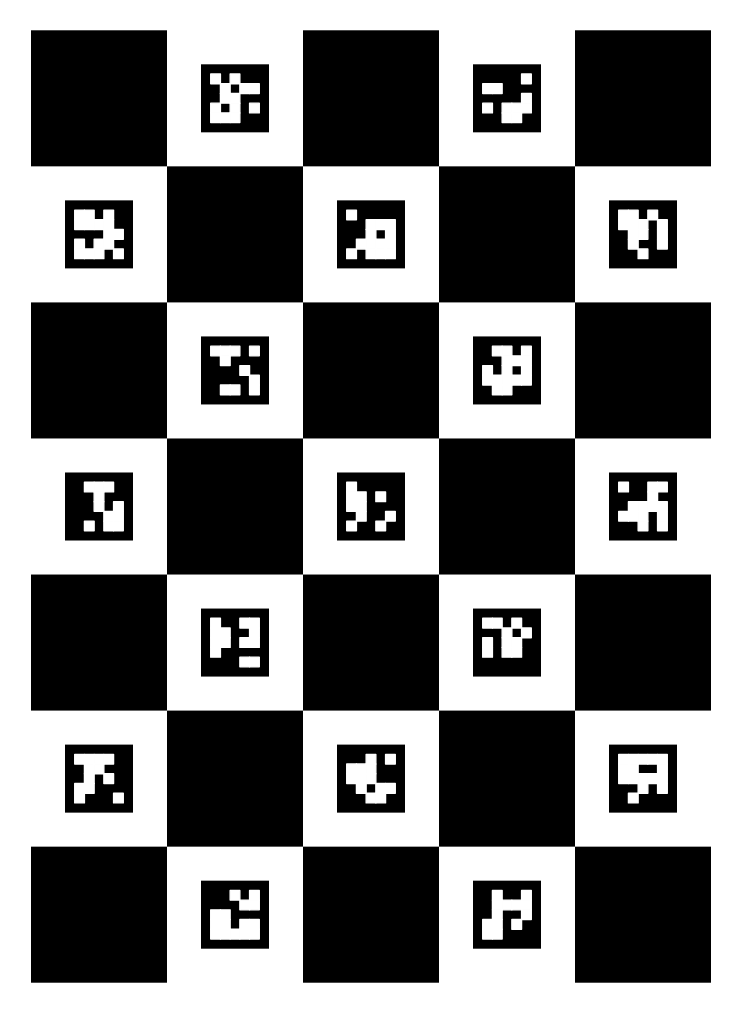
\includegraphics[width=.95\linewidth]{imgs/charuco.png}
        \caption{Example board}
    \end{subfigure}
    \begin{subfigure}{.5\textwidth}
        \centering
        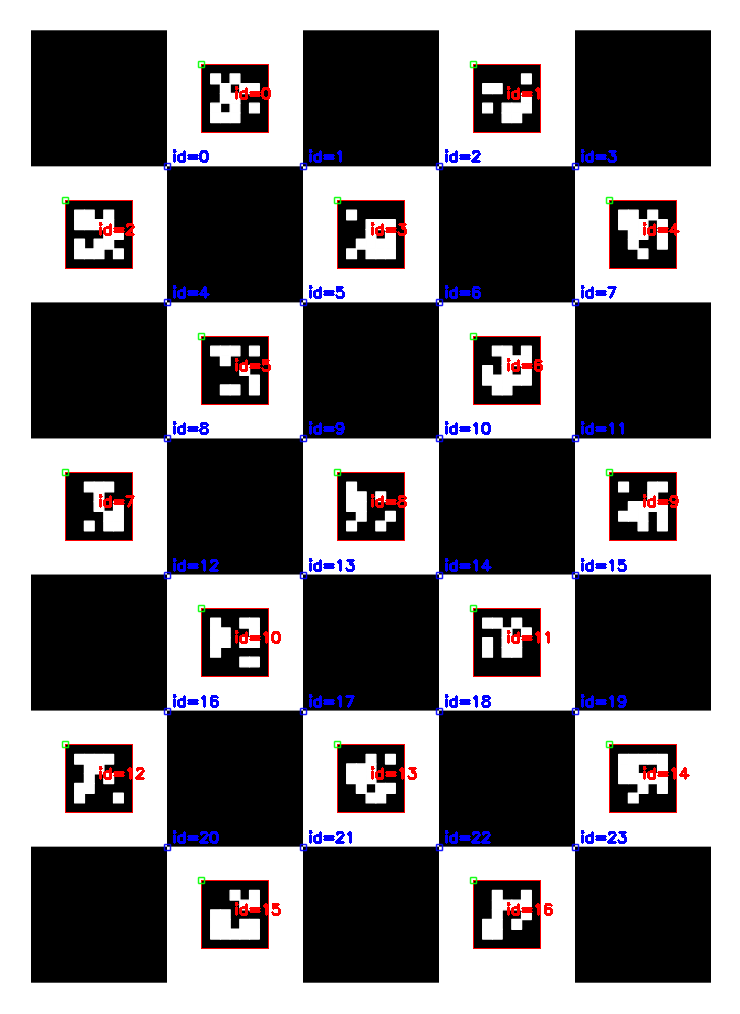
\includegraphics[width=.95\linewidth]{imgs/charucoDetect.png}
        \caption{Board with detected markers and corners drawn}
    \end{subfigure}
    \caption{ChArUco boards}
\end{figure}

\subsubsection{Zhang method for computing the intrinsic parameters}
In this subsection we will go over the math in the Zhang method for camera calibration[ref]. \\

Lets start with writing the equation correlating the 3D point to the 2D image point. The left and right matrices are the intrinsic and extrinsic matrix accordingly. The intrinsic matrix is written a bit differently than before, that's because here are we take account of skewness and aspect ratio. 
\[
    \begin{bmatrix}
    x \\
    y \\
    1 
    \end{bmatrix}
    =
    \begin{bmatrix}
    c   &   cs  &   x_H \\
    0   &   c(1+m)  &   y_H \\
    0   &   0   &   1 
    \end{bmatrix}
    \begin{bmatrix}
    r_{11}   &   r_{12}  &  r_{13}  &   t_1 \\
    r_{21}   &   r_{22}  &  r_{23}  &   t_2 \\
    r_{31}   &   r_{32}  &  r_{33}  &   t_3
    \end{bmatrix}
    \begin{bmatrix}
        X \\
        Y \\
        Z \\
        1
    \end{bmatrix}
\]
By assuming Z=0(when we use boards, all the points on the boards have the same Z=0 value) we can eliminate the 3rd column of the extrinsic matrix. 
\begin{equation}
    \begin{bmatrix}
    x \\
    y \\
    1 
    \end{bmatrix}
    =
    \begin{bmatrix}
    c   &   cs  &   x_H \\
    0   &   c(1+m)  &   y_H \\
    0   &   0   &   1 
    \end{bmatrix}
    \begin{bmatrix}
    r_{11}   &   r_{12}  &   t_1 \\
    r_{21}   &   r_{22}  &   t_2 \\
    r_{31}   &   r_{32}   &   t_3
    \end{bmatrix}
        \begin{bmatrix}
        X \\
        Y \\
        1
    \end{bmatrix}
    \label{simplifiedmappingLong}
\end{equation}
Very important thing to note is that the intrinsic parameters are the same for every image(and so every point in every image), while the extrinsic parameters are the same for every point in an image(they change from image to image). \\
We can write the transformation as a 3x3 matrix $H$. Here $K$ is the intrinsic matrix. With $H$ we can write a shorter form of \ref{simplifiedmappingLong} for every point $i$ that is on an image. 
\begin{equation}
H=[\pmb{h_1}, \pmb{h_2}, \pmb{h_3}]=K[\pmb{r_1}, \pmb{r_2}, \pmb{t}]
\label{defH}
\end{equation}

\begin{equation}
    \begin{bmatrix}
        x_i \\
        y_i \\
        1 
    \end{bmatrix}
    =
    H
    \begin{bmatrix}
        X_i \\
        Y_i \\
        1 
    \end{bmatrix}
    \quad
    i=1,...,I
    \label{simMap}
\end{equation}
From here if we would have known the extrinsic matrix we could just do a QR decomposition of $H$ and find our parameters(Q would be extrinsic, R would be intrinsic). But that is not the case. We have to find some way by using the properties of $K$ and the extrinsic matrix to extract $K$ from $H$. After that we can find the extrinsic parameters. \\
Lets start by rewriting \ref{defH} by inverting $K$. From that equation we can get equations for $r_1$ and $r_2$.
\begin{gather}
    \begin{bmatrix}
        \pmb{r_1}, \pmb{r_2}, \pmb{t}
    \end{bmatrix}
    =
    K^{-1}
    \begin{bmatrix}
        \pmb{h_1}, \pmb{h_2}, \pmb{h_3}
    \end{bmatrix}   \notag\\
    \notag\\
    \pmb{r_1}=K^{-1}\pmb{h_1} \notag\\
    \pmb{r_2}=K^{-1}\pmb{h_2}
    \label{r1r2}
\end{gather}
For the rotational vectors we know that they are orthogonal and unit vectors. Into these equations we can put the equations from \ref{r1r2}. (Note: $K^{-T}=(K^{-1})^T$ and $\|\pmb{r_1}\|=\pmb{r_1}^T \pmb{r_1}$)
\begin{gather}
    \pmb{r_1}^T \pmb{r_2}=0 \qquad \Longrightarrow \qquad \pmb{h_1}^TK^{-T}K^{-1}\pmb{h_2}=0    \notag\\
    \|\pmb{r_1}\|=\|\pmb{r_2}\|=1 \qquad \Longrightarrow \qquad \pmb{h_1}^T K^{-T}K^{-1}\pmb{h_1}-\pmb{h_2}^TK^{-T}K^{-1}\pmb{h_2}=0
    \label{hKeqs}
\end{gather}
Let us define a matrix $B$ and rewrite \ref{hKeqs}. Because $K$ only has real entries, $B$ is a positive definite matrix.
\begin{gather}
    B=K^{-T} K^{-1} \label{Bdef} \\
    \pmb{h_1}^T B \pmb{h_2}=0 \notag\\
    \pmb{h_1}^T B \pmb{h_1}-\pmb{h_2}^T B \pmb{h_2}=0
    \label{hBeqs}
\end{gather}
Notice that $B$ is a matrix times the same matrix transposed. We can find this matrix by doing a Cholesky decomposition. By doing the decomposition of $B$ our result will be the transposed inverse of $K$.
\begin{gather}
    chol(B)=A A^T   \notag\\
    A=K^{-T}
    \label{cholesky}
\end{gather}
So now if we can compute $B$ we can compute $K$. Let us write $B$ as a 3x3 symmetric matrix of unknowns and a vector $\pmb{b}$ comprised from those unknowns.
\begin{gather}
    B = \begin{bmatrix}
        b_{11} & b_{12} & b_{13} \\
        b_{12} & b_{22} & b_{23} \\
        b_{13} & b_{23} & b_{33} \\
    \end{bmatrix}   \notag\\\notag\\
    \pmb{b} = [b_{11}, b_{12}, b_{13}, b_{22}, b_{23}, b_{33}]\notag
\end{gather}
Now we rewrite \ref{hBeqs} in the form of the system $V\pmb{b}=0$(Note: $\pmb{v}_{ij}^T \pmb{b}=\pmb{h}_i^T B \pmb{h}_j$) and we get:
\begin{gather}
    \pmb{v}_{ij} = \begin{bmatrix}
        h_{i1}h_{j1},   \\
        h_{i1}h_{j2}+h_{i2}h_{j1},  \\
        h_{i3}h_{j1}+h_{i1}h_{j3},  \\
        h_{i2}h_{j2},   \\
        h_{i3}h_{j2}+h_{i2}h_{j3},  \\
        h_{i3}h_{j3}    
    \end{bmatrix}   \notag\\
    \notag\\
    \begin{bmatrix}
        \pmb{v}_{12}^T \\
        \pmb{v}_{11}^T-\pmb{v}_{22}^T
    \end{bmatrix}
    \pmb{b}=0
    \label{vsistem}
\end{gather}

Here the system is undefined because it is 2x6($\pmb{v}_{ij}$ is 1x6).  We can use n images stacking the equations and the the system becomes 2nx6. We would need 3 or more images for the system to be indefinite and we can aproximate solutions for the system by minimizing it with the constraint that $\|\pmb{b}\|=1$
\begin{gather}
    \pmb{b}^*=\min_{\pmb{b}}\|V\pmb{b}\|
    \label{bmin}
\end{gather}
With the approximation of $\pmb{b}$ we can compute the intrinsic matrix $K$

\subsubsection{Computing the extrinsic parameters}
Once we have found the intrinsic parameters $K$ we can go back and use \ref{r1r2}. We compute $\pmb{r_3}$ based on that all the rotational vectors are orthogonal and we make an equation for $\pmb{t}$ from \ref{r1r2}
\begin{gather}
    \pmb{r_1}=K^{-1}\pmb{h_1} \notag\\
    \pmb{r_2}=K^{-1}\pmb{h_2} \notag\\
    \pmb{r_3}=\pmb{r_1} \times\pmb{r_2} \notag\\
    \pmb{t}=K^{-1}\pmb{h_2} 
    \label{extrinsicequations}
\end{gather}

\subsubsection{Taking account of distortion}

As we have seen in eq. \ref{radialdistEq} and \ref{tangentialdistEq}, distortion is non linear. Our goal is to find these non linear distortion parameters $\pmb{q}$. We can implement it by introducing the positional shift(that is dependent on position $\pmb{x}$ and the distortion parameters $\pmb{q}$) to $K$. 
\[
    K^*=\begin{bmatrix}
        1   &   0   &   \Delta x(\pmb{x, q}) \\
        0   &   1   &   \Delta y(\pmb{x, q}) \\
        0   &   0   &   1
    \end{bmatrix}
    K
\]
To compute the distortion parameters we minimize the difference in position between where it needs to be and where it is for every point in every image.
\begin{equation}
    \min_{K, \pmb{q}, R_n, \pmb{t}_n}
    \sum_n  \sum_i
    \|
        \pmb{x}_{ni} - \overset{\wedge}{\pmb{x}}(K, \pmb{q}, R_n, \pmb{t}_n, \pmb{X}_{ni})
    \|^2
    \label{distMinEq}
\end{equation}

\subsubsection{Summary}
To recap here are the steps that are done to compute the intrinsic, extrinsic and distortion parameters.
\begin{enumerate}
    \item Compute $H$ from multiple images with \ref{simMap}
    \item From $H$ get $\pmb{v}_{ij}$ and calculate $\pmb{b}$ from multiple images \ref{bmin} 
    \item From $\pmb{b}$ get $\pmb{B}$, do a Cholesky decomposition, transposition and inversion and get the intrinsic matrix $K$ \ref{cholesky}
    \item From the intrinsic matrix and $H$ compute the extrinsic parameters \ref{extrinsicequations}
    \item With minimization approximate the distortion parameters \ref{distMinEq}
\end{enumerate}